\begin{figure}[!ht]
    \centering
    % \subfloat[Bayes]{
        % \label{Bayes}
        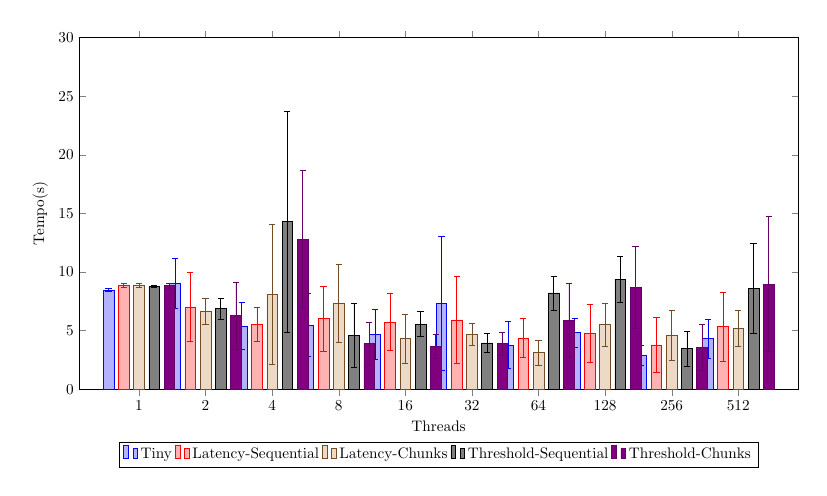
\begin{tikzpicture}[scale=0.55, baseline]
        \begin{axis}[
            width=1.5 \linewidth,
            height=0.8 \linewidth,
            %media de tempo intruder
            ybar=3pt,
            %enlargelimits=0.10,
            legend style={at={(0.5,-0.15)}, anchor=north, legend columns=-1},
            ylabel=Tempo(s),
            xlabel=Threads,
            symbolic x coords={1, 2, 4, 8, 16, 32, 64, 128, 256, 512},
            xtick=data,
            ymin=0,
            ymax=30,
            bar width=7pt,
            % nodes near coords,
            nodes near coords align={vertical},
        ]
        \addplot+[error bars,y dir=both, y explicit] coordinates {
            (1,8.46)+-(1,0.12) (2,9.04)+-(2,2.15) (4,5.41)+-(4,2.01) (8,5.49)+-(8,2.70) (16,4.71)+-(16,2.14) (32,7.33)+-(32,5.74) (64,3.78)+-(64,1.99) (128,4.82)+-(128,1.20) (256,2.87)+-(256,0.84) (512,4.32)+-(512,1.69)
        };
        \addplot+[error bars,y dir=both, y explicit] coordinates {
            (1,8.86)+-(1,0.17) (2,7.02)+-(2,2.95) (4,5.52)+-(4,1.47) (8,6.03)+-(8,2.78) (16,5.75)+-(16,2.44) (32,5.92)+-(32,3.68) (64,4.36)+-(64,1.66) (128,4.78)+-(128,2.50) (256,3.78)+-(256,2.36) (512,5.34)+-(512,2.97)
        };
        \addplot+[error bars,y dir=both, y explicit] coordinates {
            (1,8.87)+-(1,0.14) (2,6.68)+-(2,1.10) (4,8.09)+-(4,5.99) (8,7.33)+-(8,3.29) (16,4.32)+-(16,2.09) (32,4.71)+-(32,0.94) (64,3.12)+-(64,1.09) (128,5.50)+-(128,1.87) (256,4.62)+-(256,2.12) (512,5.18)+-(512,1.52)
        };
        \addplot+[error bars,y dir=both, y explicit] coordinates {
            (1,8.80)+-(1,0.10) (2,6.87)+-(2,0.90) (4,14.29)+-(4,9.42) (8,4.60)+-(8,2.73) (16,5.56)+-(16,1.06) (32,3.95)+-(32,0.79) (64,8.22)+-(64,1.45) (128,9.40)+-(128,1.98) (256,3.48)+-(256,1.49) (512,8.61)+-(512,3.82)
        };
        \addplot+[error bars,y dir=both, y explicit] coordinates {
            (1,8.84)+-(1,0.21) (2,6.29)+-(2,2.84) (4,12.79)+-(4,5.91) (8,3.91)+-(8,1.84) (16,3.66)+-(16,1.03) (32,3.89)+-(32,0.97) (64,5.88)+-(64,3.19) (128,8.70)+-(128,3.51) (256,3.60)+-(256,1.96) (512,8.97)+-(512,5.75)
        };
        \legend {Tiny, Latency-Sequential, Latency-Chunks, Threshold-Sequential, Threshold-Chunks}
        \end{axis}
        \end{tikzpicture}
    % }
    \caption{Tempo de execução em segundos do benchmark Bayes variando o número de \emph{threads}.}
    \label{bayes_tmp}

\end{figure}
